% ════════════════════════════════════════════════════════════════
\subsection{Dowód optymalności algorytmu Huffmana}
% ════════════════════════════════════════════════════════════════

Kody prefiksowe $\iff$ regularne drzewa binarne.

$C$ -- alfabet, $f: C \to \N$ funkcja częstości, $d_T(c)$ -- głębokość liścia reprezentującego $c$ w drzewie $T$ reprezentującym kod prefiksowy.
\begin{flalign*}
	B(T) = \sum_{c\in C} f(c) \cdot d_T(c) \longleftarrow \min &  &  &  &
\end{flalign*}

\begin{lemma} \label{lemma:huffman:1}
	Niech $x$ i $y$ będą najrzadziej występującymi znakami z $C$. Istnieje optymalny kod prefiksowy, w którym słowa kodowe $x$ i $y$ mają tę samą długość i różnią się tylko na ostatnim bicie.
\end{lemma}

Z lematu~\ref{lemma:huffman:1} wynika, że można zacząć konstrukcję optymalnego drzewa połączeniem dwóch symboli o najmniejszej częstości.
\textbf{Zachłanny wybór} -- w każdym kroku algorytm łączy dwa wierzchołki o najmniejszych kluczach.

\begin{lemma} \label{lemma:huffman:2}
	Niech $A$ będzie alfabetem z funkcją częstości $f: A \to \N$, a $x, y \in A$ — dwoma znakami o najmniejszych częstościach. Zdefiniujmy zredukowany alfabet $A' = (A \setminus \{x, y\}) \cup \{z\}$, gdzie $z \notin A$, z funkcją częstości $f'$ taką, że $f'(c) = f(c)$ dla $c \neq z$ oraz $f'(z) = f(x) + f(y)$.

	Jeśli $T'$ jest optymalnym drzewem kodu prefiksowego dla $(A', f')$, to drzewo $T$ powstałe z $T'$ przez zastąpienie liścia $z$ wewnętrznym węzłem z dziećmi $x$ i $y$ jest optymalnym drzewem kodu prefiksowego dla $(A, f)$.
\end{lemma}

\begin{center}
	\begin{tikzpicture}[
			leaf/.style={draw=none, font=\small},
			inner/.style={circle, draw, minimum size=0.5cm, inner sep=0pt}]

		% ===== T' =====
		\begin{scope}
			\draw (-1,0) -- (1,0) -- (0,1.5) -- cycle;     % pozostała część drzewa
			\node[leaf] (zp) at (0,-1.1) {$z$};
			\draw (0,0) -- (zp);
			\node[leaf] at (0,-2.4) {$T'$};
		\end{scope}

		% ===== strzałka =====
		\node[leaf, font=\large] at (2.6,-0.4) {$\Rightarrow$};

		% ===== T =====
		\begin{scope}[xshift=5.2cm]
			\draw (-1,0) -- (1,0) -- (0,1.5) -- cycle;     % pozostała część drzewa
			\node[inner] (p) at (0,-0.9) {};
			\draw (0,0) -- (p);
			\node[leaf] (x) at (-0.65,-1.9) {$x$};
			\node[leaf] (y) at (0.65,-1.9) {$y$};
			\draw (p) -- (x);
			\draw (p) -- (y);
			\node[leaf] at (0,-2.4) {$T$};
		\end{scope}
	\end{tikzpicture}
\end{center}

\begin{theorem}
	Algorytm Huffmana konstruuje drzewo reprezentujące optymalny kod prefiksowy.
\end{theorem}

% ════════════════════════════════════════════════════════════════
\subsection{Szeregowanie zadań}
% ════════════════════════════════════════════════════════════════

\begin{problem}[Szeregowanie zadań -- jeden procesor]
Jak uszeregować zadania tak, aby średni czas ukończenia był jak najmniejszy?
\end{problem}

\begin{example}[Szeregowanie zadań -- jeden procesor] \label{prob:szeregowanieZadan}
	\leavevmode
	\begin{table}[H]
		\centering
		\renewcommand{\arraystretch}{1.2}
		\begin{NiceTabular}{c|c|c}[margin,hvlines]
			$i$ & zadanie & $t_i$ \\
			\hline
			1   & $z_1$   & 15    \\
			2   & $z_2$   & 8     \\
			3   & $z_3$   & 3     \\
			4   & $z_4$   & 10
		\end{NiceTabular}
	\end{table}

	Rozważmy uszeregowanie $z_1, z_2, z_3, z_4$:
	\begin{flalign*}
		\frac{15 + (15+8) + (15+8+3) + (15+8+3+10)}{4} = \frac{15 + 23 + 26 + 36}{4} = \frac{100}{4} = 25 &  &  &  &
	\end{flalign*}

	Rozważmy uszeregowanie $z_3, z_2, z_4, z_1$:
	\begin{flalign*}
		\frac{3 + (3+8) + (3+8+10) + (3+8+10+15)}{4} = \frac{3 + 11 + 21 + 36}{4} = 17 \frac{3}{4} &  &  &  &
	\end{flalign*}

	\textbf{Rozwiązanie:} Uszereguj zadania od najkrótszego do najdłuższego.
\end{example}

\begin{problem}[Szeregowanie zadań -- 3 procesory] \label{prob:szeregowanieZadanTrzy}
Mamy 3 procesory. Pytanie jak poprzednio (por. \ref{prob:szeregowanieZadan}).
\end{problem}

\begin{example}[Szeregowanie zadań -- trzy procesory]
	\leavevmode
	\begin{table}[H]
		\centering
		\renewcommand{\arraystretch}{1.2}
		\begin{NiceTabular}{c|c|c|c|c|c|c|c|c|c}[margin,hvlines]
			Zadanie & $z_1$ & $z_2$ & $z_3$ & $z_4$ & $z_5$ & $z_6$ & $z_7$ & $z_8$ & $z_9$ \\
			\hline
			$t_i$   & 3     & 5     & 6     & 10    & 11    & 14    & 15    & 18    & 20
		\end{NiceTabular}
	\end{table}

	\textbf{Rozwiązanie:} Przydzielaj zadania do pierwszego wolnego procesora w kolejności od najkrótszego do najdłuższego.

	\begin{figure}[H]
		\centering
		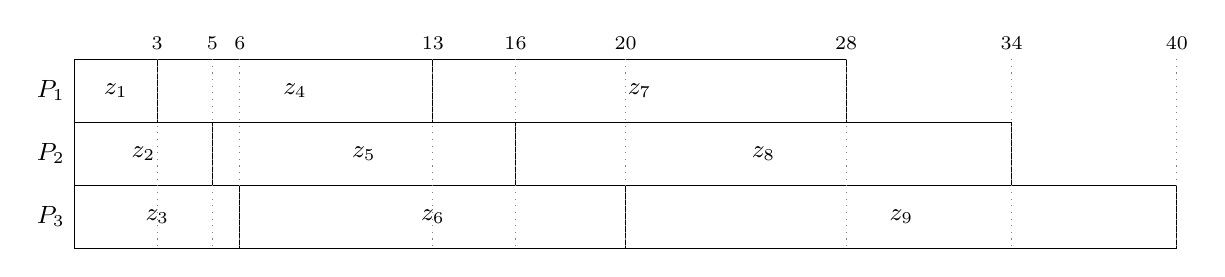
\begin{tikzpicture}[x=0.35cm, y=0.8cm, font=\small]
			% P1
			\draw (0, 2) rectangle (3, 3) node[midway] {$z_1$};
			\draw (3, 2) rectangle (13, 3) node[midway] {$z_4$};
			\draw (13, 2) rectangle (28, 3) node[midway] {$z_7$};

			% P2
			\draw (0, 1) rectangle (5, 2) node[midway] {$z_2$};
			\draw (5, 1) rectangle (16, 2) node[midway] {$z_5$};
			\draw (16, 1) rectangle (34, 2) node[midway] {$z_8$};

			% P3
			\draw (0, 0) rectangle (6, 1) node[midway] {$z_3$};
			\draw (6, 0) rectangle (20, 1) node[midway] {$z_6$};
			\draw (20, 0) rectangle (40, 1) node[midway] {$z_9$};

			\node[left] at (0, 2.5) {$P_1$};
			\node[left] at (0, 1.5) {$P_2$};
			\node[left] at (0, 0.5) {$P_3$};

			\foreach \x in {3, 5, 6, 13, 16, 20, 28, 34, 40} {
					\node[above, font=\scriptsize] at (\x, 3) {\x};
					\draw[gray, dotted] (\x, 3) -- (\x, 0);
				}
		\end{tikzpicture}
	\end{figure}
\end{example}

W problemie \ref{prob:szeregowanieZadan} dla uszeregowania $z_{i_1}, z_{i_2}, \dots, z_{i_n}$ suma zakończeń zadań wynosi:
\begin{flalign*}
	\sum_{j=1}^n \sum_{k=1}^j t_{i_k} & = t_{i_1} + (t_{i_1} + t_{i_2}) + (t_{i_1} + t_{i_2} + t_{i_3}) + \dots + (t_{i_1} + \dots + t_{i_n}) =            &  & \\
	                                  & = n \cdot t_{i_1} + (n - 1) t_{i_2} + (n - 2) t_{i_3} + \dots + 1 \cdot t_{i_n} = \sum_{j=1}^n (n + 1 - j) t_{i_j} &  &
\end{flalign*}

W problemie \ref{prob:szeregowanieZadanTrzy} (dla $3 \mid n$) dla uszeregowania $z_{i_1}, z_{i_2}, \dots, z_{i_n}$ suma czasów zakończeń wynosi:
\begin{flalign*}
	\vphantom{\sum_{j=1}^n \left( \frac{n}{3} - \left\lfloor \frac{j-1}{3} \right\rfloor \right)} & \underbracket{t_{i_1} + t_{i_2} + t_{i_3}} + \underbracket{(t_{i_1} + t_{i_4}) + (t_{i_2} + t_{i_5}) + (t_{i_3} + t_{i_6})} + \underbracket{(t_{i_1} + t_{i_4} + t_{i_7}) + (t_{i_2} + t_{i_5} + t_{i_8}) + (t_{i_3} + t_{i_6} + t_{i_9})} + &  & \\
	\vphantom{\sum_{j=1}^n \left( \frac{n}{3} - \left\lfloor \frac{j-1}{3} \right\rfloor \right)} & + \dots + \underbracket{(t_{i_1} + t_{i_4} + \dots + t_{i_{n-2}}) + (t_{i_2} + t_{i_5} + \dots + t_{i_{n-1}}) + (t_{i_3} + t_{i_6} + \dots + t_{i_n})} =                                                                                     &  & \\
	\vphantom{\sum_{j=1}^n \left( \frac{n}{3} - \left\lfloor \frac{j-1}{3} \right\rfloor \right)} & = \frac{n}{3} (t_{i_1} + t_{i_2} + t_{i_3}) + \left(\frac{n}{3} - 1\right) (t_{i_4} + t_{i_5} + t_{i_6}) + \left(\frac{n}{3} - 2\right) (t_{i_7} + t_{i_8} + t_{i_9}) + \dots + 1 \cdot (t_{i_{n-2}} + t_{i_{n-1}} + t_{i_n}) =              &  & \\
	                                                                                              & = \sum_{j=1}^n \left( \frac{n}{3} - \left\lfloor \frac{j-1}{3} \right\rfloor \right) t_{i_j} = \sum_{j=1}^n \left\lceil \frac{n+1-j}{3} \right\rceil \cdot t_{i_j}                                                                           &  &
\end{flalign*}

\begin{lemma}
	Niech $A_1 \geq A_2 \geq \dots \geq A_n$. Dla dowolnej permutacji $\Pi = (i_1, \dots, i_n)$ zbioru $[n]$ niech $f(\Pi) = \sum_{j=1}^n A_j \cdot t_{i_j}$. Wtedy $f$ osiąga minimum na każdej permutacji ustawiającej czasy niemalejąco, tzn. takiej, że $t_{i_1} \leq t_{i_2} \leq \dots \leq t_{i_n}$.
\end{lemma}

\begin{conclusion}
	Nasze algorytmy szeregowania zadań są poprawne.
\end{conclusion}
